\documentclass{article}
\usepackage[utf8]{inputenc}
\usepackage{graphicx}

\title{Climate uncertainty as an integral part of IAMs}
\author{Chris Smith}
\date{June 2022}

\begin{document}

\maketitle

\section{Introduction}

Process-based integrated assessment models (IAMs) such as MESSAGE, REMIND, GCAM, AIM/CGE, WITCH and IMAGE provide emissions pathways for climate emulators for assessment of mitigation pathways for the IPCC Working Group 3 assessment report (Kikstra et al., Riahi et al.). Climate assessment via emulators is the last step of the process chain that starts with exogenous inputs of population, urbanisation, education and GDP storylines provided by the shared socioeconomic pathways. The IAM is the energy-economy model sitting in between, solving an optimisation problem that (for example) maximises utility given the exogenous boundary conditions, subject to constraints surrounding technological deployment. In the real world, energy supply, energy demand and human decision making is likely to be a function of climate change, as is economic development with consequential effects on climate damages that lowers GDP growth (Rising et al. 2022). A few process-based IAMs have the capability to use climate data in their energy-economic model (ref WITCH ex., IMAGE ex., GCAM ex), but even where the capability exists climate change is not explicitly considered within IAM-derived scenarios submitted to the IPCC Working Group 3 database. As far as climate is implicitly used as a constraint it is limited to solving for a total remaining carbon budget (REF) or year-2100 radiative forcing target (REF ScenarioMIP). The former makes heavy assumptions on the linearity and time-independence of warming with cumulative CO$_2$ emissions, and the latter relies on post-hoc assessments of emissions pathways and is limited to merely checking that the scenario  has approximately the target forcing (Gidden et al. 2019). 

Neither of these approximate implicit climate constraints take into account how climate uncertainty could affect the optimal solution of an IAM pathway. Despite recent advances, large uncertainties still exist in assessments of aerosol radiative forcing (Bellouin et al 2020), climate sensitivity (Sherwood et al. 2020), the transient response to cumulative CO$_2$ emissions (Canadell et al. 2021) and zero emissions commitment (Lee et al. 2021); the latter two parameters strongly influencing the remaining carbon budget (Rogelj et al. 2019). in the real world, adaptation and mitigation effort is not likely to be independent of climate dynamics. If it turns out that climate sensitivity is high and climate is warming faster than expected, mitigation action may be ramped up in order to avoid even higher levels of warming.

We use a simple cost-benefit IAM, the Dynamic Integrated model of Climate and the Economy (DICE2016R; Nordhaus et al. a, b, c, d...), as a proof of concept to show that climate uncertainty is critically important on the emissions projections, temperature, and social cost of carbon in so-called ``optimal'' pathways that maximise utility. DICE is a global model and does not include sectoral assumptions, and is structually much simpler than a processed-based IAM, but does include a climate damage function that reduces consumption and hence utility, and so does include a climate-economy feedback that the SSP framework does not permit. DICE's simplicity also permits large ensembles given its short run time, in common with the climate emulators typically used to assess IAM emissions scenarios.

It has been noted by several authors (Dietz et al. 2021; Folini et al. 2022; Gasser et al. 2022) that the climate emulator component of the DICE model and other cost-benefit IAMs (FUND, PAGE) perform poorly compared to observations or the behaviour Earth System models in their default configuration. We therefore couple the economic model of DICE with the carbon cycle and climate response from FaIR (Millar et al. 2017; Smith et al. 2018; Leach et al. 2021), specifically the version used to assess IAM pathways from the IPCC's Working Group 3 report (Riahi et al. 2022; Byers et al. 2022; Kikstra et al. 2022). Using this calibrated, observationally constrained probabilistic calibration of FaIR (Smith et al. 2021), we run 2237 ensemble members in DICE, systematically varying the carbon cycle feedback, climate response (including climate sensitivity), non-CO$_2$ radiative forcing strengths assuming an SSP2-4.5 forcing pathway, and observational uncertainty on near-present-day (2015) warming. The default configuration of the DICE2016R economic model is unchanged.

%Constraints on the FaIR ensemble include reproducing observed historical warming from 1850-2019 to a root-mean-squared error of less than 0.135°C, and close correspondence with distributions from IPCC assessments of 1995-2014 warming relative to 1850-1900, atmospheric CO$_2$ concentrations in 2014; aerosol radiative forcing in 2005-2014; equilibriium climate sensitivity; transient climate repsonse; transient climate response to CO$_2$ emissions; and future warming projections for SSP scenarios (Forster et al. 2021; Smith et al. 2021).

We show that resulting emissions pathways consistent with optimal maximisation of utility in DICE vary substantially (fig. \ref{fig:projections}a), showing a range of compatible CO$_2$ fossil fuel emissions in the range of 4 to 42 GtCO$_2$ yr$^{-1}$ in 2100. Variation in the emissions pathways coupled with varying strengths of carbon cycle feedbacks to temperature and cumulative CO$_2$ emissions (fig. \ref{fig:projections}b). This ``optimal'' pathway results in 3°C (2.5-3.5°C) of warming by the end of the century (fig. \ref{fig:projections}c), though we caution that climate damages may be severely underestimated in DICE (REF) and no policy-relevant temperature constraints have been implemented such as a commitment to limit warming well below 2°C, which would easily be possible to test the feasibility of. Finally, the social cost of carbon also shows large variability, ranging from X to Y \$ tCO$_2^{-1}$ in 2020 and increasing exponentially over the next 100 years (fig. \ref{fig:projections}d). We remark that substitution of the default climate module of DICE with FaIR results in lower median warming projections and lower levels of the social cost of carbon than in the original DICE model (Nordhaus et al. 2017), the climate component of which has been shown to respond to emissions too quickly (Folini et al. 2022; Gasser et al. 2022).

\begin{figure}
\centering
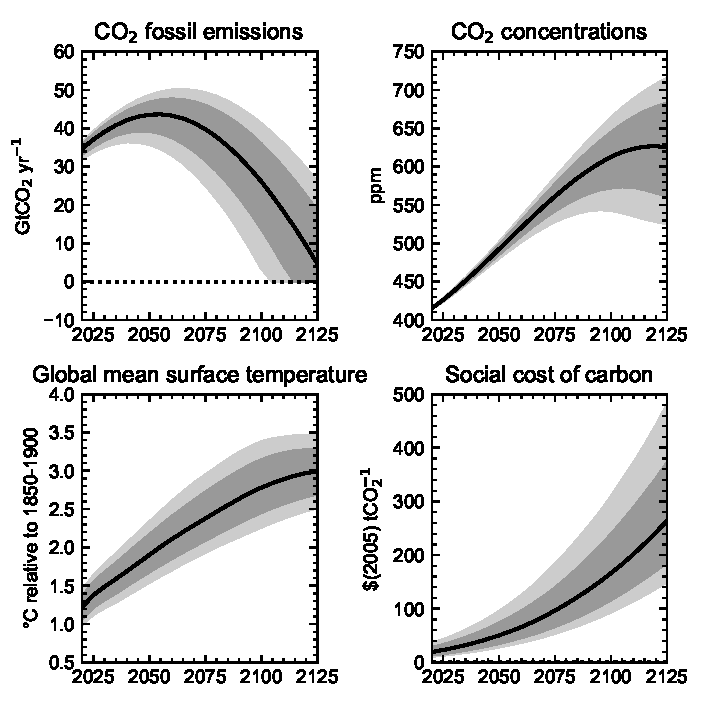
\includegraphics[width=12cm]{../../figures/climate_projections.pdf}
\caption{Projections of (a) fossil fuel CO$_2$ emissions; (b) atmospheric CO$_2$ concentrations; (c) global mean temperature projections; (d) social cost of carbon using the constrained, calibrated probabilistic ensemble of FaIR from the IPCC Sixth Assessment Report coupled to the economic model of DICE. Light shaded bands show 5-95\% range; dark shaded range show 16-84\% range; black lines show ensemble medians.}
\label{fig:projections}
\end{figure}

This proof-of-concept can be used in scenario development, for example to address implausibility concerns about high warming scenarios such as SSP5-8.5 achieving continued GDP growth that outpaces increasingly severe climate damages (Woodard et al. 2019). Future work will seek to incorporate climate feedbacks and uncertainty into a process-based IAM. It would also be possible to design an ensemble that calculated the social cost of carbon for a well-below 2°C scenario by stipulating that 66\% or 90\% of ensemble members had to remain below this threshold, to conduct a sensitivity analysis to determine the main climatic factors contributing to the uncertainty in the social cost of carbon, and to combine climate uncertainty with economic uncertainty.

\end{document}
